%% LyX 2.0.2 created this file.  For more info, see http://www.lyx.org/.
%% Do not edit unless you really know what you are doing.
\documentclass[english,review]{acmsiggraph}
\usepackage[T1]{fontenc}
\usepackage[latin9]{inputenc}
\usepackage{amssymb}
\usepackage{graphicx}

\makeatletter
%%%%%%%%%%%%%%%%%%%%%%%%%%%%%% User specified LaTeX commands.
% for the following cases use the listed document class option:
% [annual] - Technical paper accepted for presentation at the ACM SIGGRAPH 
%   or SIGGRAPH Asia annual conference.
% [sponsored] - Short or full-length technical paper accepted for 
%   presentation at an event sponsored by ACM SIGGRAPH
%   (but not the annual conference Technical Papers program).
% [abstract] - A one-page abstract of your accepted content
%   (Technical Sketches, Posters, Emerging Technologies, etc.). 
%   Content greater than one page in length should use the "[sponsored]"
%   parameter.
% [preprint] - A preprint version of your final content.
% [review] - A technical paper submitted for review. Includes line
%   numbers and anonymization of author and affiliation information.

% When you submit your paper for review, please use the \TOGonlineID''
% command to include the online ID value assigned to your paper by the
% submission management system. Replace '45678' with the value you were
% assigned.
\TOGonlineid{XXXXX}

% If you are preparing a preprint of your accepted paper, and your paper
% will be published in an issue of the ACM "Transactions on Graphics''
% journal, replace the "0'' values in the commands below with the correct
% volume and number values for that issue - you'll get them before your
% final paper is due.
\TOGvolume{0}
\TOGnumber{0}

% The TOGarticleDOI' command accepts the DOI information provided to you
% during production, and which makes up the URLs which identifies the ACM
% article page and direct PDF link in the ACM Digital Library.
% Replace "1111111.2222222'' with the values you are given.
\TOGarticleDOI{1111111.2222222}

% If you would like to include links to personal repositories for auxiliary
% material related your research contribution, you may use one or more of
% these commands to define an appropriate URL. The "\TOGlinkslist'' command
% found just before the first section of your document will add hyperlinked
% icons to your document, in addition to hyperlinked icons which point to
% the ACM Digital Library article page and the ACM Digital Library-held PDF.
\TOGprojectURL{}
\TOGvideoURL{}
\TOGdataURL{}
\TOGcodeURL{}

% Paper title.
\title{Shape Enhanced With and Adapted Laplacian Operator For Hybrid Quad/Triangle Meshes}

% Author and Affiliation (single author).
%\author{Name \thanks{e-mail: name@unknown.uu}\\ Research Institute}

% Author and Affiliation (multiple authors).
\author{Alexander Pinzon\thanks{e-mail: apinzonf@gmail.com}
\qquad  Eduardo Romero\thanks{e-mail:edromero@unal.edu.co}
 \\Cimalab Research Group\\National University of Colombia}
%\and Ton Roosendaal\thanks{e-mail:ton@blender.org}\\ Blender CEO}

% The ``pdfauthor'' command accepts the authors of the work,
% comma-delimited, and adds this information to the PDF metadata.
%\pdfauthor{Alexander Pinzon, Eduardo Romero, Ton Roosendaal}
\pdfauthor{Anonymous}

% Keywords that describe your work.
\keywords{laplacian smooth, curvature, sculpting, subdivision surface}

\makeatother

\usepackage{babel}
\begin{document}







\teaser{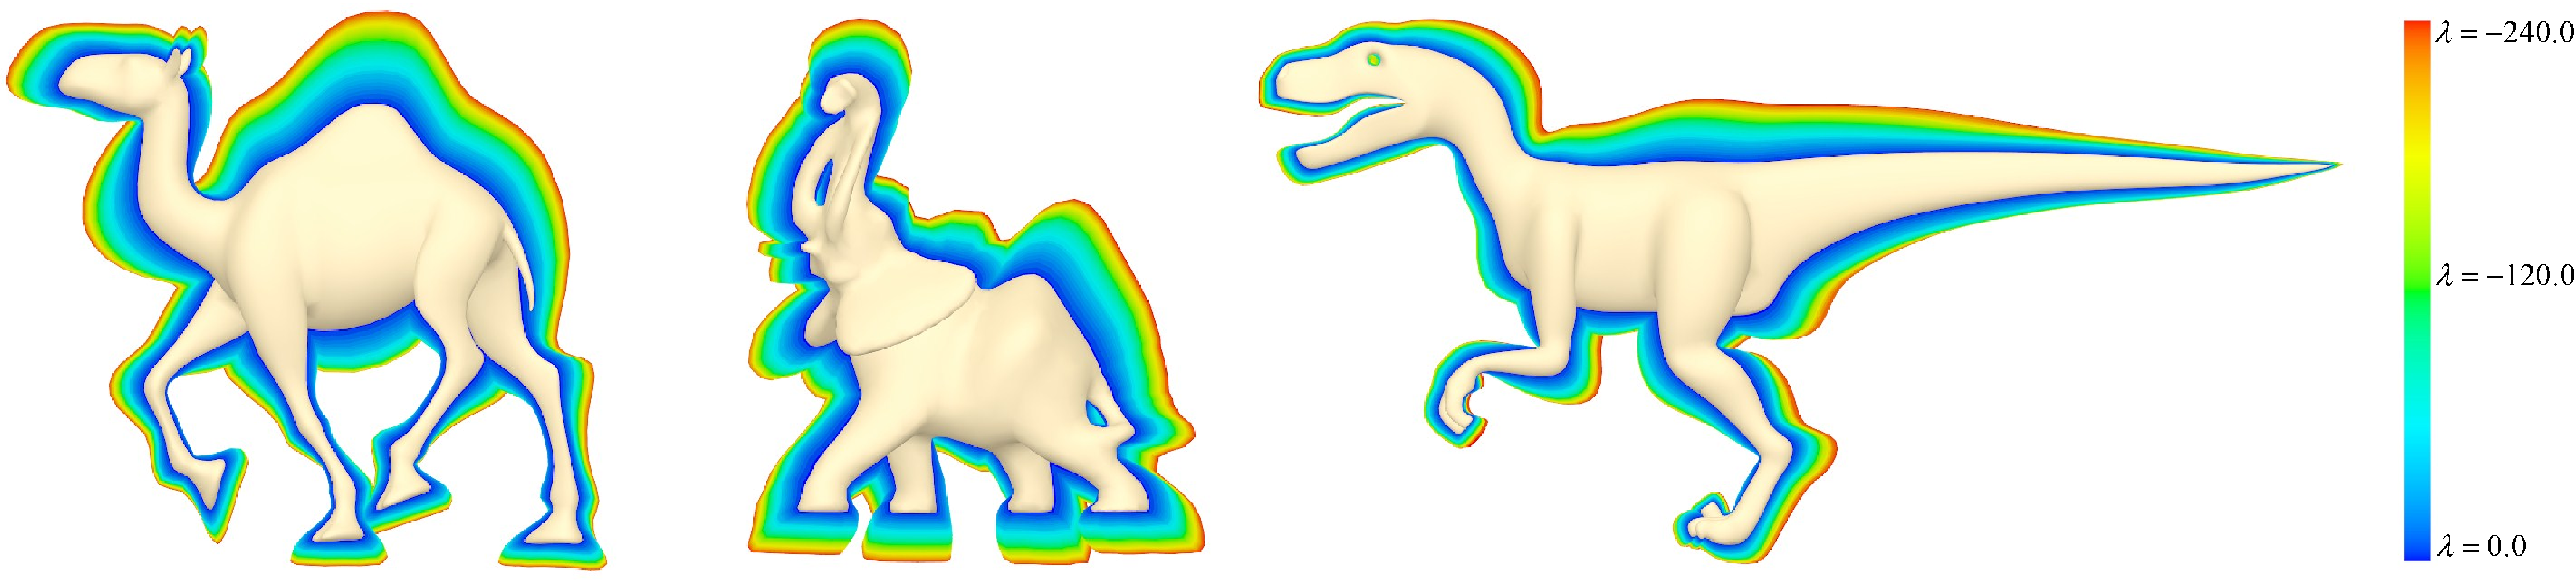
\includegraphics[width=1\textwidth]{images/spectrum} \caption{\label{fig:Spectrum}A set of 48 successive shapes enhanced, from
$\lambda=0.0$ in blue to $\lambda=-240.0$ in red, with steps of
$-5.0$.}
}

\maketitle
\maketitle 
\begin{abstract}
This paper proposes a novel modeling method for a hybrid quad/triangle
mesh that allows to set a family of possible shapes by controlling
a single parameter, the global curvature. The method uses an original
extension of the Laplace Beltrami operator that efficiently estimates
a curvature parameter which is used to define an enhanced shape after
a particular operation performed in certain mesh points. Along with
the method, this work presents new applications in sculpting and modeling,
with subdivision of surfaces and weight vertex groups. A series of
graphics examples demonstrates the quality, predictability and flexibility
of the method in a real production environment with software Blender.
\end{abstract}

\begin{CRcatlist}
\CRcat{I.3.5}{Computer Graphics}{Computational Geometry and Object Modeling
}{Modeling packages}
\end{CRcatlist}
\keywordlist

\TOGlinkslist

%\copyrightspace


\section{Introduction}

Over the last years several, modeling techniques able to generate
a variety of realistic shapes, have been developed \cite{Botsch2006}.
Editing techniques have evolved from affine transformations to advanced
tools like sculpting \cite{Coquillart1990,Galyean1991,Stanculescu2011},
editing, creation from sketches \cite{Igarashi1999,Gonen2012}, and
complex interpolation techniques \cite{Sorkine2004,Zhou2005}. Catmull-Clark
based methods however require to interact with a minimun number of
control points for any operation to be efficient, or in other words,
a unicity condition is introduced by demanding a smooth surface after
any of these shape operations. Hence, traditional modeling methods
for subdividing surfaces from coarse geometry have become widely popular
\cite{Catmull1978,Stam1998}. These works have generalized a uniform
B-cubic spline knot insertion to meshes, some of them adding some
type of control, for instance with the use of creases to produce sharp
edges \cite{DeRose1998}, or the modification of some vertex weights
to locally control the zone of influence \cite{Biermann2000}. Neverteless
these methods are difficult to deal with since they require a large
number of parameters and a very tedious customization. Instead, the
presented method requires a single parameter that controls the global
curvature, which is used to maintain realistic shapes, creating a
family of different versions of the same object and therefore preserving
the detail of the original model and a realistic appearance. 

Interest in meshes composed of triangles and quads has lately increased
because of the flexibility of modeling tools such as Blender 3D \cite{blender}.
Nowadays, many artists use a manual connection of a couple of vertices
to perform animation processes and interpolation \cite{Mullen2007}.
It is then of paramount importance to develop operators that easily
interact with such meshes, eliminating the need of preprocessing the
mesh to convert it to triangles. The shape enhancement and shape exaggeration
can thus be used as such brush in the sculpting process, when inflating
a shape since current brushes end up by losing detail when moving
vertices \cite{Stanculescu2011}. In contrast, the presented method
inflates a mesh by moving the vertices towards the reverse curvature
direction, conserving the shape and sharp features of the model.

\textbf{Contributions} This work presents an extension of the Laplace
Beltrami operator for hybrid quad/triangle meshes, representing a
larger mesh spectrum from what has been presented so far. The method
eliminates the need of preprocessing and allows preservation of the
original topology. Likewise, along with this operator, it is proposed
a method to generate a family of parameterized shapes, in a robust
and predictable way. This method enables customization of the smoothness
and curvature, obtained during the subdivision surfaces process. Finally,
it is proposed a new brush for enhancing the silhouette mesh features
in modeling and sculpting.

This work is organized as follows: Section \ref{sub:1.1-Related-work}
presents works related to the Laplacian mesh processing, digital sculpting,
and offsetting methods for polygonal meshes; In section \ref{sec:Laplacian-Smooth}
, it is described the theoretical framework of the Laplacian operator
for polygon meshes; In section \ref{sec:Proposed-Method}, it is presented
the method for shape enhancement and applications of subdivision of
surfaces and sculpting; finally some Laplacian operator results, to
hybrid quad/triangle meshes are graphically shown as well as results
of the shape enhancement applications in sculpting, subdivision and
modeling.


\section{Related work\label{sub:1.1-Related-work}}

Many tools have been developed for modeling, based on the Laplacian
mesh processing. Thanks to the advantages of the Laplacian operator,
these different tools preserve the surface geometric details when
using them for different processes such as free-form deformation,
fusion, morphing and other applications \cite{Sorkine2004}. 

Offset methods for polygon meshing, based on the curvature defined
by the Laplace Beltrami operator, have been developed. These methods
adjust the shape offset by a constant distance, with enough precision
as to minimize the Hausdorff error. Nevertheless, these methods fail
to conserve sufficient detail because of the smoothing, a crucial
issue which depends on the offset size \cite{Zhuo2012}. In volumetric
approaches, in case of point-based representations, the offset boundary
computation is based on the distance field and therefore when calculating
such offset, the topology of the model may be different to the original
\cite{Chen2011}.

\cite{Gal2009} propose automatic feature detection and shape edition
with feature inter-relationship preservation. They define salient
surface features like ridges and valleys, characerized by their first
and second order curvature derivatives \cite{Ohtake2004}, and angle-based
threshold. Likewise, curves have been also classified as planar or
non-planar, approximated by lines, circles, ellipses and other complex
shapes. In such case, the user defines an initial change over several
features which is propagated towards other features, based on the
classified shapes and the inter-relationships between them. This method
works well with objects that have sharp edges, composed of basic geometric
shapes such as lines, circles or ellipses. However, the method is
very limited when models are smooth since it cannot find the proper
features to edit.

Digital sculpting have been traditionally approached either under
a polygonal representation or a voxel grid-based method. Brushes for
inflation operations only depend on the vertex normal \cite{Stanculescu2011}.
In grid-based sculpting, some other operations have allowed to add
or remove voxels since production of polygonal meshes require a processing
of isosurfaces from a volume \cite{Galyean1991}. The drawback comes
from the difficulty of maintaining the surface details during larger
scale deformations.


\section{Laplacian Smooth\label{sec:Laplacian-Smooth}}

\begin{figure*}[t]
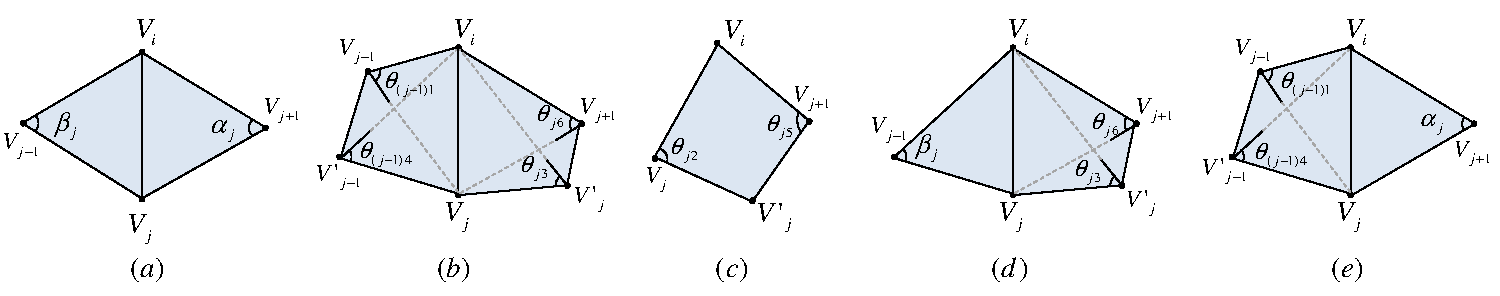
\includegraphics[width=1\textwidth]{images/beltrami}

\caption{\label{fig:LBO-basic-5-TQ}The 5 basic triangle-quad cases with common
vertex $V_{i}$ and the relationship with $V_{j}$ and $V_{j}^{\prime}$.
(a) Two triangles {[}Desbrun 1999{]}. (b) (c) Two quads and one quad
{[}Xiong 2011{]}. (d) (e) Triangles and quads (TQLBO).}
\end{figure*}


Computer objects, reconstructed from the real world, are usually noisy.
Laplacian Smooth techniques allow a proper noise reduction on the
mesh surface with minimal shape changes, while still preserving a
desirable geometry as well as the original shape. 

Many smoothing Laplacian functionals regularize the surface energy
by controling the total surface curvature $S$.

\begin{equation}
E\left(S\right)=\int_{S}\kappa_{1}^{2}+\kappa_{2}^{2}dS\label{eq:total_cuarvature_integral}
\end{equation}


Where $\kappa_{1}$ and $\kappa_{2}$ are the two principal curvatures
of the surface $S$.


\subsection{Gradient of Voronoi Area}

\begin{figure}[h]
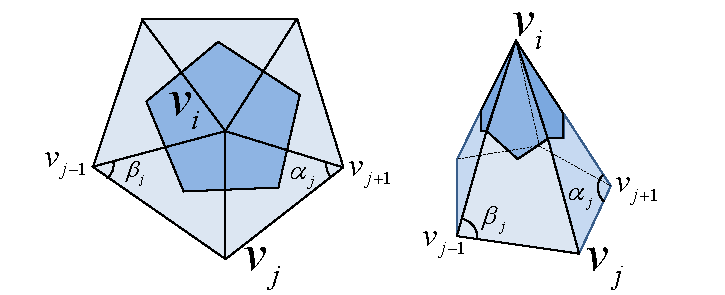
\includegraphics[width=1\columnwidth]{images/voronoi_region}

\caption{\label{fig:voronoi_region}Area of the Voronoi region around $v_{i}$
in dark blue.\protect \\
 $v_{j}$ belong to the first neighborhood around $v_{i}$. $\alpha_{j}$
and $\beta_{j}$ opposite angles to edge $\protect\overrightarrow{v_{j}-v_{i}}$. }
\end{figure}


Consider a surface $S$ composed of a set of triangles around vertex
$v_{i}$. Let us define the \textit{Voronoi region} of $v_{i}$ as
show in figure \ref{fig:voronoi_region}, The area change produced
by the movement of $v_{i}$ is called the gradient of \textit{Voronoi
region \cite{Pinkall1993,Desbrun1999,Meyer2003}.}

\begin{equation}
\nabla A=\frac{1}{2}\underset{j}{\sum}\left(\cot\alpha_{j}+\cot\beta_{j}\right)\left(v_{i}-v_{j}\right)\label{eq:eq_gradient_voronoi_area}
\end{equation}


If the gradient in equation (\ref{eq:eq_gradient_voronoi_area}) is
normalized by the total area of the $1$-ring neighborhood around
$v_{i}$, the \textit{discrete mean curvature normal} of a surface
$S$ is obtained, as shown in equation (\ref{eq:discrete_mean_curvature_normal}).

\begin{equation}
2\kappa\mathbf{n}=\frac{\nabla A}{A}\label{eq:discrete_mean_curvature_normal}
\end{equation}



\subsection{Laplace Beltrami Operator}

The \textit{Laplace Beltrami operator} LBO noted as $\triangle_{g}$
is used for measuring the mean curvature normal to the Surface $S$
\cite{Pinkall1993}. 

\begin{equation}
\triangle_{g}S=2\kappa\mathbf{n}\label{eq:def_LBO}
\end{equation}


The LBO has desirable properties: the LBO points out to the direction
of the minimal surface area, minimizing the energy of the total surface
curvature $S$ at equation (\ref{eq:total_cuarvature_integral}).


\section{Proposed Method\label{sec:Proposed-Method}}

This method exaggerates a shape using a Laplacian smoothing operator
in the reverse direction, i.e., the new shape is a modified version
in which those areas with larger curvature are magnified. The operator
amounts to a generator of a set of models which conserves the basic
silhouette of the original shape. In addition, the presented approach
can be easily mixed with traditional or uniform subdivision of surfaces.
This method is based on an original extension of the Laplace Beltrami
operator for hybrid quad/triangle meshes, mixing arbitrary types of
meshes, exploiting the basic geometrical relationships and ensuring
algorithm convergence. 


\subsection{Laplace Beltrami Operator for Hybrid Quad/Triangle Meshes TQLBO\label{sub:Laplace-Beltrami-operator}}

Given a mesh $M=\left(V,Q,T\right)$, with vertices $V$, quads $Q$,
triangles $T$. The area of $1$-ring neighborhood $A\left(v_{i}\right)$
corresponds to a sum of the quad faces $A\left(Q_{v_{i}}\right)$
and the areas of the triangular faces $\ensuremath{A\left(T_{v_{i}}\right)}$
adjacent to vertex $\ensuremath{v_{i}}$.

\begin{center}
$A\left(v_{i}\right)=A\left(Q_{v_{i}}\right)+A\left(T_{v_{i}}\right)$.
\par\end{center}

\begin{figure}[h]
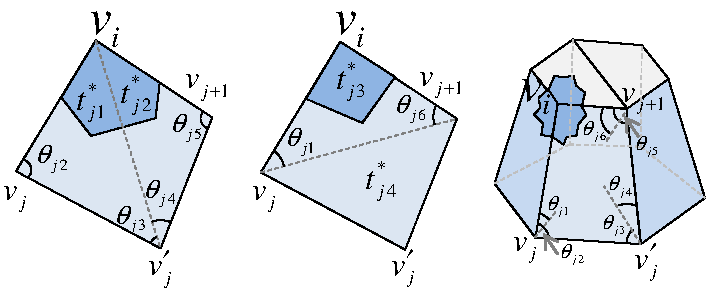
\includegraphics[width=1\columnwidth]{images/quad_xiong}

\caption{\label{fig:quad_xiong}$t_{j1}^{*}\equiv\vartriangle v_{i}v_{j}v_{j}^{\prime},\, t_{j2}^{*}\equiv\vartriangle v_{i}v_{j}^{\prime}v_{j+1},\, t_{j3}^{*}\equiv\vartriangle v_{i}v_{j}v_{j+1}$
Triangulations of the quad with common vertex $v_{i}$ proposed by
{[}Xiong 2011{]} to define Mean LBO.}
\end{figure}


Applying the mean average area, according to \cite{Xiong2011}, from
all possible triangulations, as show in figure \ref{fig:quad_xiong},
the area for quads $\ensuremath{A\left(Q_{v_{i}}\right)}$ and triangles
$A\left(T_{v_{i}}\right)$ is.

\begin{center}
$A\left(v_{i}\right)=\frac{1}{2^{m}}\overset{m}{\underset{j=1}{\sum}}2^{m-1}A\left(q_{j}\right)+\overset{r}{\underset{k=1}{\sum}}A\left(t_{k}\right)$
\par\end{center}

Where $q_{1},q_{2},...,q_{j},...,q_{m}\in Q_{v_{i}}$ and $t_{1},t_{2},...,t_{k},...,t_{r}\in T_{v_{i}}$.

\begin{equation}
A\left(v_{i}\right)=\frac{1}{2}\overset{m}{\underset{j=1}{\sum}}\left[A\left(t_{j1}^{*}\right)+A\left(t_{j2}^{*}\right)+A\left(t_{j3}^{*}\right)\right]+\overset{r}{\underset{k=1}{\sum}}A\left(t_{k}\right)\label{eq:area_1_ring_triangles_quads}
\end{equation}


Applying the gradient operator to (\ref{eq:area_1_ring_triangles_quads}).

{\small 
\begin{equation}
\nabla A\left(v_{i}\right)=\frac{1}{2}\overset{m}{\underset{j=1}{\sum}}\left[\nabla A\left(t_{j1}^{*}\right)+\nabla A\left(t_{j2}^{*}\right)+\nabla A\left(t_{j3}^{*}\right)\right]+\overset{r}{\underset{k=1}{\sum}}\nabla A\left(t_{k}\right)\label{eq:EqGrad}
\end{equation}
}{\small \par}

According to (\ref{eq:eq_gradient_voronoi_area}), we have.

\begin{center}
$\nabla A\left(t_{j1}^{*}\right)=\frac{\cot\theta_{j3}\left(v_{j}-v_{i}\right)+\cot\theta_{j2}\left(v_{j}^{\prime}-v_{i}\right)}{2}$
\par\end{center}

\begin{center}
$\nabla A\left(t_{j2}^{*}\right)=\frac{\cot\theta_{j5}\left(v_{j}^{\prime}-v_{i}\right)+\cot\theta_{j4}\left(v_{j+1}-v_{i}\right)}{2}$
\par\end{center}

\begin{center}
$\nabla A\left(t_{j3}^{*}\right)=\frac{\cot\theta_{j6}\left(v_{j}-v_{i}\right)+\cot\theta_{j1}\left(v_{j+1}-v_{i}\right)}{2}$
\par\end{center}

\begin{center}
$\nabla A\left(t_{k}\right)=\frac{\cot\alpha_{k}\left(v_{k}-v_{i}\right)+\cot\beta_{k+1}\left(v_{k+1}-v_{i}\right)}{2}$
\par\end{center}

Triangle and quad configurations of the 1-ring neighborhood faces,
adjacent to $v_{i}$, can be simplified to five cases, as shown in
figure \ref{fig:LBO-basic-5-TQ}.

According to equation (\ref{eq:discrete_mean_curvature_normal}),
(\ref{eq:def_LBO}), and five simple cases defined in figure \ref{fig:LBO-basic-5-TQ}
the TQLBO (Triangle-Quad LBO) of $v_{i}$ is.

\begin{equation}
\triangle_{g}\left(v_{i}\right)=2\kappa\mathbf{n}=\frac{\nabla A}{A}=\underset{v_{j}\in N_{1}\left(v_{i}\right)}{\frac{1}{2A}\sum}w_{ij}\left(v_{j}-v_{i}\right)
\end{equation}


{\small 
\begin{equation}
w_{ij}=\begin{cases}
\left(\cot\alpha_{j}+\cot\beta_{j}\right) & \mbox{case }\mathit{a.}\\
\frac{1}{2}\left(\cot\theta_{\left(j-1\right)1}+\cot\theta_{\left(j-1\right)4}+\cot\theta_{j3}+\cot\theta_{j6}\right) & \mbox{case \ensuremath{\mathit{b}}.}\\
\left(\cot\theta_{j2}+\cot\theta_{j5}\right) & \mbox{case \ensuremath{\mathit{c}}.}\\
\frac{1}{2}\left(\cot\theta_{j3}+\cot\theta_{j6}\right)+\cot\beta_{j} & \mbox{case \ensuremath{\mathit{d}}.}\\
\frac{1}{2}\left(\cot\theta_{\left(j-1\right)1}+\cot\theta_{\left(j-1\right)4}\right)+\cot\alpha_{j} & \mbox{case \ensuremath{\mathit{e}}.}
\end{cases}\label{eq:TQLBO_wij}
\end{equation}
}{\small \par}

We define a Laplacian operator as a matrix equation

\begin{equation}
L\left(i,j\right)=\begin{cases}
-\frac{1}{2A_{i}}w_{ij} & \mbox{if }j\in N\left(v_{i}\right)\\
\frac{1}{2A_{i}}\underset{j\in N\left(v_{i}\right)}{\sum}w_{ij} & \mbox{if }i=j\\
0 & \mbox{otherwise}
\end{cases}\label{eq:TQLBO_Simple_Matrix}
\end{equation}


Where $L$ is a $n\times n$ matrix, $n$ is the number of vertices
of a given mesh $M$, $w_{ij}$ is the TQLBO defined in equation (\ref{eq:TQLBO_wij}),
$N\left(v_{i}\right)$ is the 1-ring neighborhood with shared face
to $v_{i}$, $A_{i}$ is the ring area around $v_{i}$.

Normalized version of the TQLBO as a matrix equation

\begin{equation}
L\left(i,j\right)=\begin{cases}
-\frac{w_{ij}}{\underset{j\in N\left(v_{i}\right)}{\sum}w_{ij}} & \mbox{if }j\in N\left(v_{i}\right)\\
\delta_{ij} & \mbox{otherwise}
\end{cases}\label{eq:TQLBO-Normalized_Matrix}
\end{equation}


Where $\delta_{ij}$ being the Kronecker delta function.


\subsection{The Shape Enhancement\label{sub:Curvature-Enhancing}}

\begin{figure*}[t]
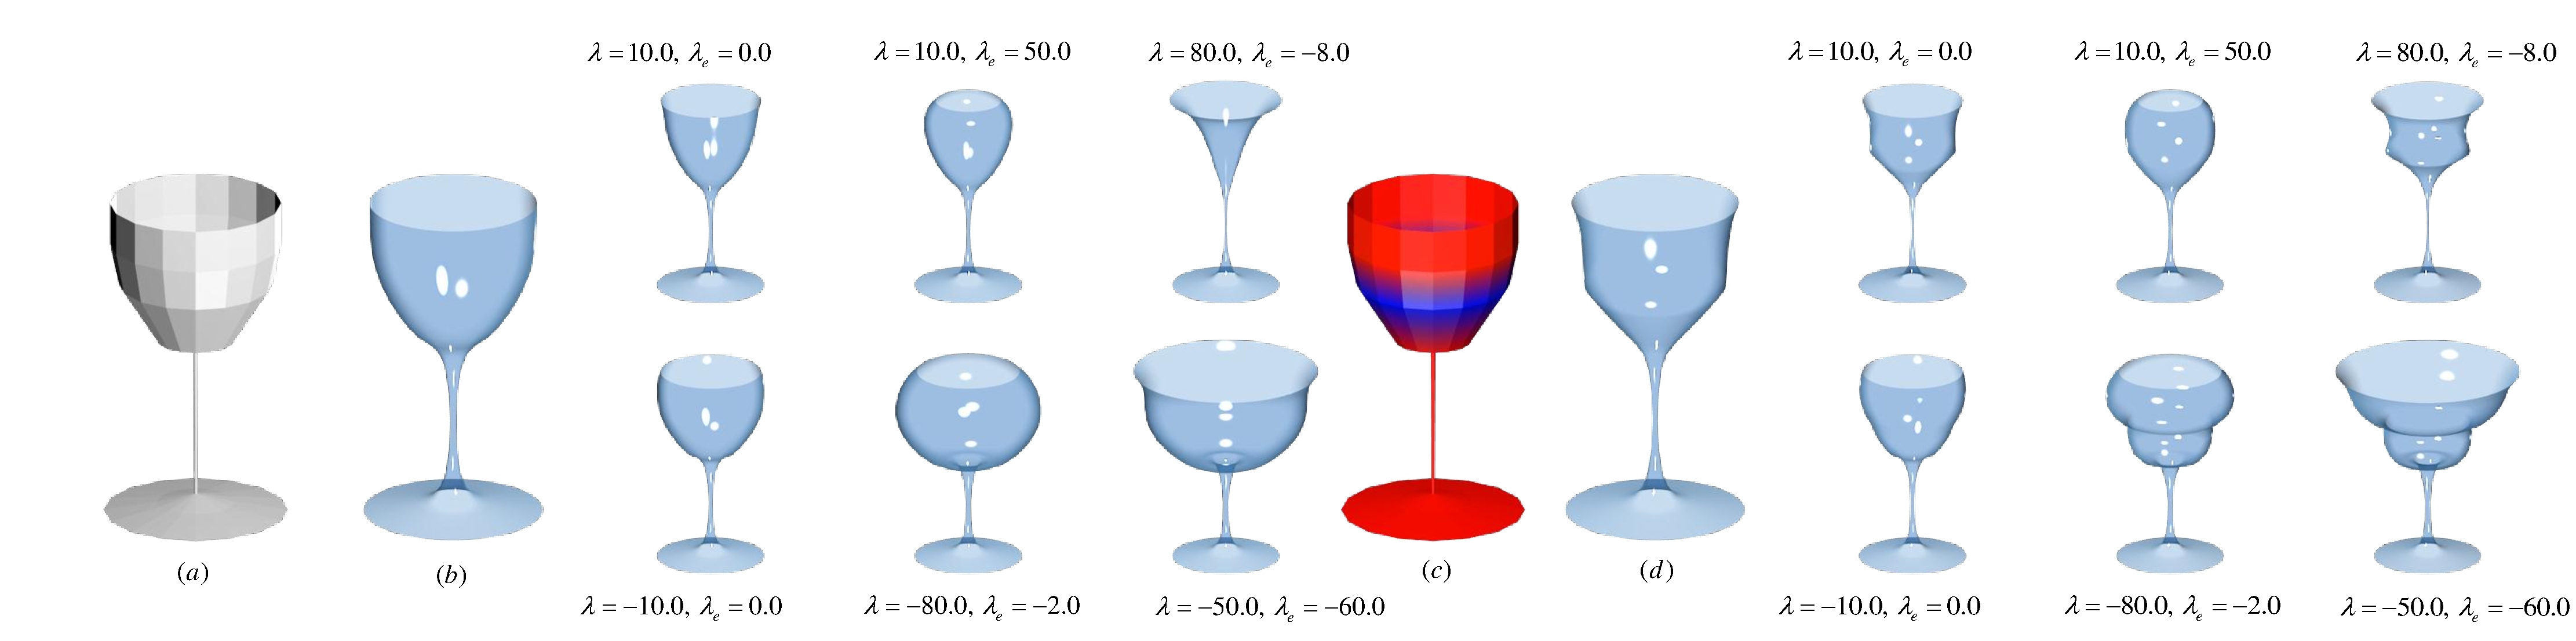
\includegraphics[width=1\textwidth]{images/teaser_cup}

\caption{\label{fig:Subdivision-Cups} Family of cups generated with our method,
from a coarse model (a), (c): the shape, obtained from the Catmull-Clark
Subdivision (b), (d), is enhanced. Soft constraints, over the coarse
model, is drawn in red and blue (c).}


\end{figure*}


The shape is enhanced by using the reverse direction of the curvature
flow, moving the vertices towards those mesh portions with larger
curvature. A standard diffusion process is applied:

\begin{center}
$\frac{\partial V}{\partial t}=\lambda L\left(V\right)$ 
\par\end{center}

To solve this equation, implicit integration is used as well as a
normalized version of TQLBO matrix.

\begin{equation}
\left(I-\left|\lambda dt\right|W_{p}L\right)V^{\prime}=V^{t}\label{eq:Lineal_System_with_wp}
\end{equation}


\begin{center}
$V^{t+1}=V^{t}+\mbox{sign}\left(\lambda\right)\left(V^{\prime}-V^{t}\right)$
\par\end{center}

The vertices $V^{t+1}$ are enhanced, along their reverse curvature
direction, by solving the linear system: $Ax=b$, where $A=I-\left|\lambda dt\right|W_{p}L$,~
$L$ is the Normalized TQLBO defined in the equation (\ref{eq:TQLBO-Normalized_Matrix}),
$x=V^{\prime}$ are the smoothing vertices, $b=V^{t}$ are the actual
vertices positions, $W_{p}$ is a diagonal matrix with weight vertex
group, and $\lambda dt$ is the enhancement factor that supports negative
and positive values: negative for enhancement and positive for smoothing. 

The method was devised to use with weighted vertex groups, which specify
the final shape enhancement of the solution, meaning $0$ as no changes
and 1 when a maximal change is applied. The weights modify the influence
zones, where the Laplacian is applied, as shown in equation \ref{eq:Lineal_System_with_wp}.
Interestingly, the generated family of shapes may change substantially
with the weights of specific control points.

The curvature cannot be calculted at the boundary of the meshes that
are not closed, for that reason we use the scale-dependent operator
proposed by Desbrun et al. \cite{Desbrun1999}, the enhancement factor
for boundary is represented by $\lambda_{e}$.

The model volume increases as the lambda is larger and negative, this
can be counteracted with a simple volume preservation. However, the
mesh may suffer large displacements when $\lambda<-1.0$ or after
multiple iterations. A simple volume conservation algorithm is: If
$v_{i}^{t+1}$ is a mesh vertex of $V^{t+1}$ in the $t+1$ iteration,
we define $\overline{v}$ as:

\begin{center}
$\overline{v}=\frac{1}{n}\underset{v_{i}\in V}{\sum}v_{i}$, 
\par\end{center}

$\overline{v}$ is the mesh center, $vol_{ini}$ is an initial volume,
and $vol_{t+1}$ is the volume at the iteration $t+1$, then the scale
factor.

\begin{center}
$\beta=\left(\frac{vol_{ini}}{vol_{t+1}}\right)^{\frac{1}{3}}$
\par\end{center}

allows to scale the vertices to:

\begin{center}
$v_{i\, new}^{t+1}=\beta\left(v_{i}^{t+1}-\overline{v}\right)+\overline{v}$
\par\end{center}


\subsection{Sculpting\label{sub:Sculpting}}

\begin{figure*}[t]
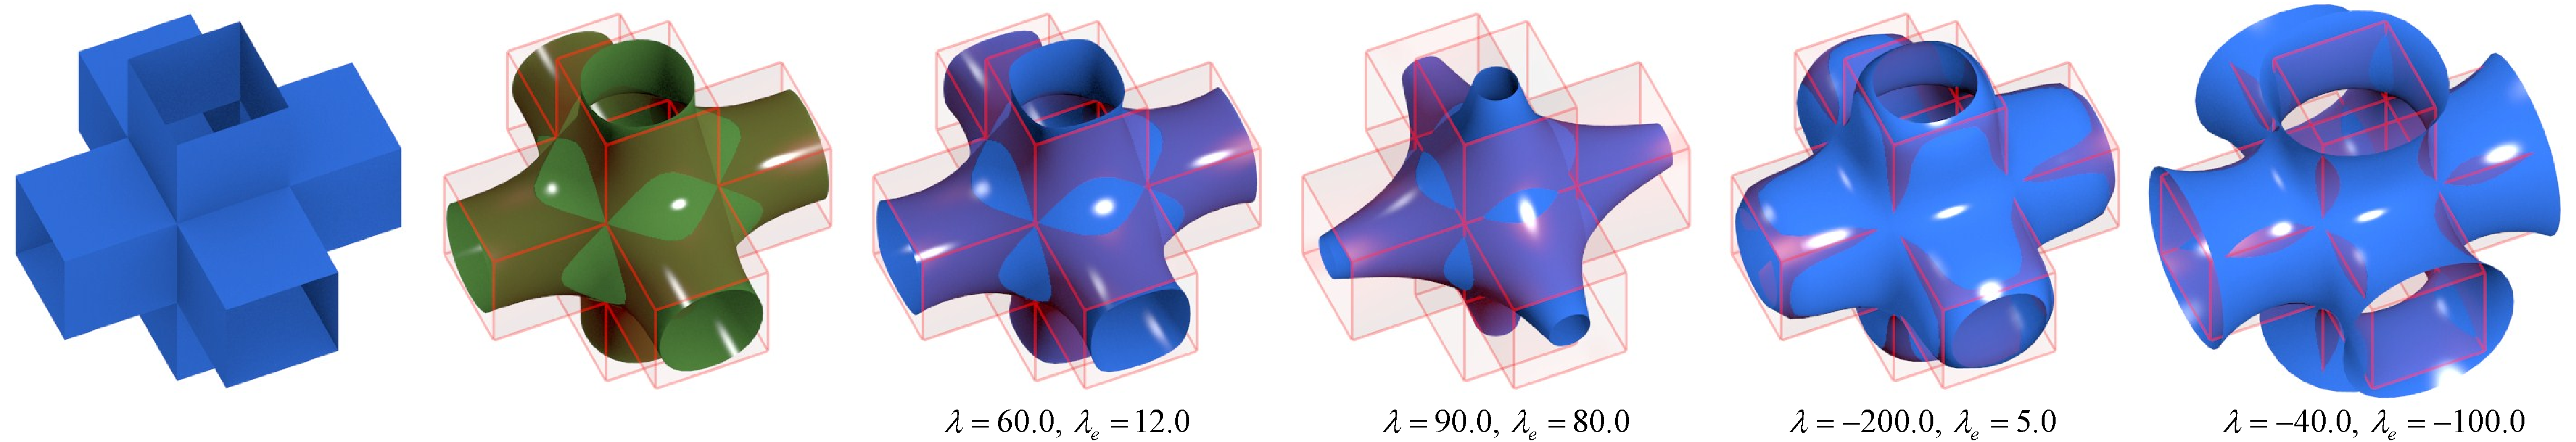
\includegraphics[width=1\textwidth]{images/cruz_lambda4}

\caption{\label{fig:Catmull_Clark}(a) Original Model, (b) Model with Catmull-Clark
Subdivision. Models with Laplacian smoothing: (c) and (d). Models
with a first Laplacian filtering $\lambda=60.0$, $\lambda_{e}=12.0$
and before applying shape enhancement: (e) and (f).}
\end{figure*}


A new sculpting brush is herein proposed and aims to inflate the shape,
magnifying the shape curvatures of a polygon mesh in real time. This
brush works properly with the stroke method \textsl{Drag Dot}, allowing
to pre-visualize the model changes before the mouse is released. Also,
it allows to move the mouse along the model to match the shape zone
which is supposed to be enhanced.

Brushes that perform a similar inflation can introduce mesh distortions
or produce mesh self-intersections, provided these brushes only move
the vertices along the normal without any global information. In contrast,
the present method searches for a proper inflation while preserving
the global curvature, retaining the original shape and main model
features. In addition, this method simplifies the work required for
the enhancement since it needs not different brushes for inflating,
softening or styling. The enhanced brush can make all these operation
in a single step. Real-time brushes require the Laplacian matrix is
constructed with the vertices that are within the sphere radius defined
by the user, reducing the matrix to be processed, the center of this
sphere depending on the place where the user clicks on the canvas
and the three-dimensional mesh placed where the click is projected.
Special handling is required for the boundary vertices with neighbors
that are not within the brush radius: these vertices are marked as
boundary and the curvature is not there calculated, but they must
be included in the matrix so that every vertex has their corresponding
neighbors within the selection. The sculpting Laplacian matrix reads
as.

\begin{center}
$L\left(i,j\right)=\begin{cases}
-\frac{w_{ij}}{\underset{j\in N\left(v_{i}\right)}{\sum}w_{ij}} & \mbox{if }\left\Vert v_{i}-u\right\Vert <r\wedge\left\Vert v_{j}-u\right\Vert <r\\
0 & \mbox{if }\left\Vert v_{i}-u\right\Vert <r\wedge\left\Vert v_{j}-u\right\Vert \geq r\\
\delta_{ij} & \mbox{otherwise}
\end{cases}$
\par\end{center}

Where $v_{j}\in N\left(v_{i}\right)$, $u$ is the sphere center of
radius $r$. The matrices should remove rows and columns of vertices
that are not within the radius.


\subsection{Subdivision surfaces\label{sub:Subdivision-surfaces}}

The Catmull-Clark subdivision transformation is used to smooth a surface,
as the limit of a sequence of subdivision steps \cite{Stam1998}.
This process is governed by a B-spline curve \cite{Loop1987}, performing
a recursive subdivision transformation that refines the model into
a linear interpolation that approximates a smooth surface. The model
smoothness is automatically guaranteed \cite{DeRose1998}. 

Catmull-Clark subdivision surface methods generate smooth and continuous
models from a coarse model and produce quick results because of the
simplicity of implementation. Nevertheless, changes to the global
curvature are hardly implantable. The Catmull-Clark subdivision surfaces
together with shape enhancement can easily generate families of shapes
by changing a single parameter, allowing to handle a model with very
few vertices. In practice, this would allow an artist to choose a
model from a similar set of options that would meet his/her needs
without having to change each of the control vertices. Likewise, the
presented method allows the use of vertex weight paint over the control
points. The weights can be applied to a coarse model, followed by
a Catmull-Clark subdivision where weights are interpolated, producing
weights with smooth changes in the influence zones, as shown in figure
\ref{fig:Subdivision-Cups}.c.

In equation \ref{eq:Lineal_System_with_wp}, $W_{p}$ is a diagonal
matrix with weights corresponding to each vertex. Weights at each
vertex produce a different solution so that the matrix must be placed
in the diffusion equation since families that are generated may change
substantially with weighted of specific control points.


\section{Results\label{sec:Results}}

The results of the shape enhancement method with the extension of
the Laplace Beltrami operator for hybrid quad/triangle meshes with
several example models (see figures \ref{fig:Spectrum}, \ref{fig:Subdivision-Cups},
\ref{fig:Catmull_Clark}, \ref{fig:TQLBO_test}, \ref{fig:camello_enhanced},
\ref{fig:Sculpt_Brush}, \ref{fig:Performance-sculpt}, \ref{fig:(a)Monkey},
\ref{fig:Animated_Camell}). The shape enhancement was assessed with
TQLBO method on a PC with AMD Quad-Core Processor @ 2.40 GHz and 8
GB RAM.

Figure \ref{fig:TQLBO_test} shows the results when applying the Laplace
Beltrami Operator TQLBO of equation (\ref{eq:TQLBO_Simple_Matrix})
in a model with a simple subdivision. In column (c) the Laplacian
smoothing was applied to a model consisting of only quads. In column
(d) the model was converted to triangles and then the Laplacian smoothing
was applied. In column (e) the model was randomly converted from some
quads into triangles and then the Laplacian smoothing is applied,
showing similar results to those meshes composed only of triangles
or quads.

\begin{figure}
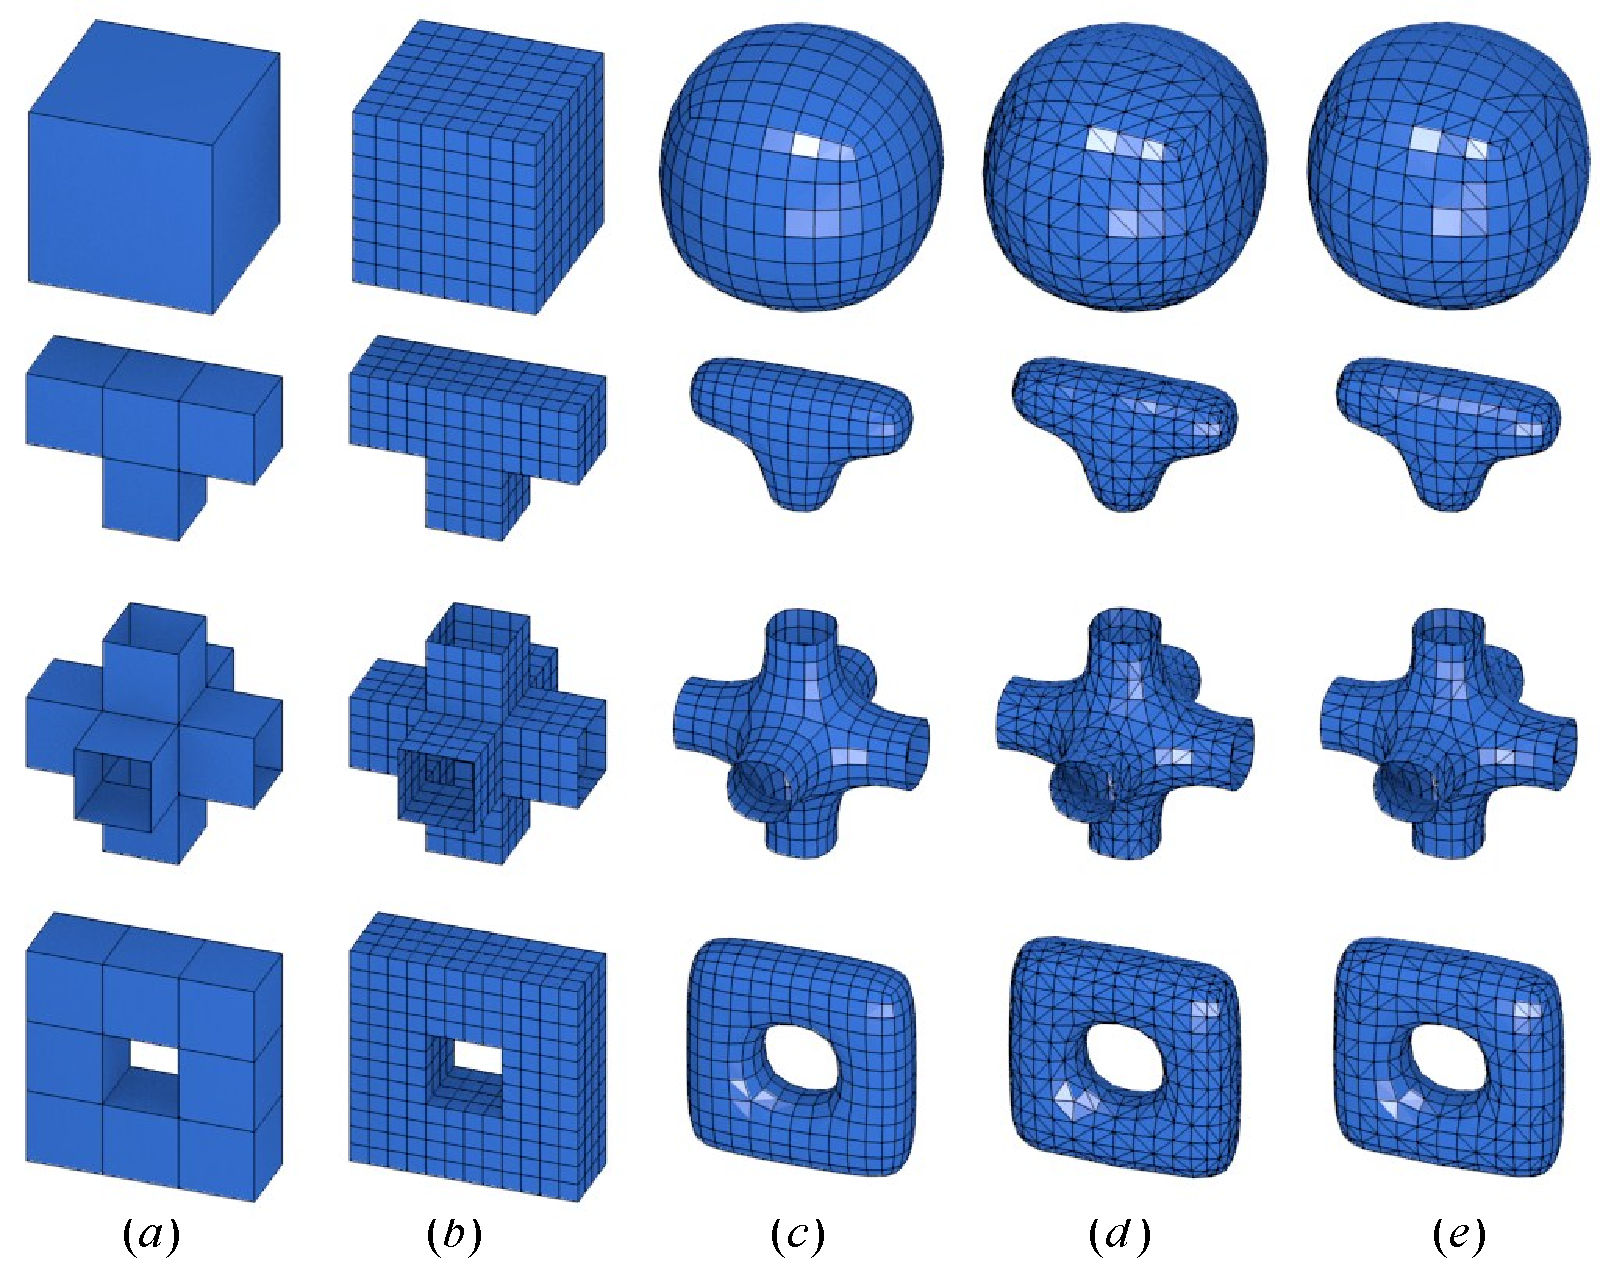
\includegraphics[width=1\columnwidth]{images/test_triangles_quads}

\caption{\label{fig:TQLBO_test}(a) Original Model. (b) Simple subdivision.
(c), (d) (e) Laplacian smoothing with $\lambda=7$ and 2 iterations:
(c) for triangles, (d) for quads, (e) for triangles and quads random
chosen.}
\end{figure}


Methods using the Catmull-Clark subdivision surface and the enhancement
allows to modify the curvature that is obtained with the process of
subdivision, as shown in figure \eqref{fig:Subdivision-Cups}. This
test used a coarse cup model, in which the subdivision was performed,
followed by a Laplacian smoothing and enhancement. In figure \eqref{fig:Subdivision-Cups}.c,
\eqref{fig:Subdivision-Cups}.d shows also the use of weight vertex
groups over coarse models, with subdivision surfaces that allowed
to generate the weights for the new interpolated vertices. These new
weights were used for the enhancement obtained on the 6 cups that
are at the right of the figure \eqref{fig:Subdivision-Cups}.d.

Laplacian smoothing applied with simple subdivision (see figure \ref{fig:Catmull_Clark}.b.)
may produce similar results to those obtained with Catmull-Clark (see
figure \ref{fig:Catmull_Clark}.c.), whose models are in average equal
triangles. The one obtained with the Laplacian smoothing is shown
in panel (c), (d) and those curvature modified versions are in (e)
and (f). As can be observed, different versions of the original sketch
can be obtained by parameterizing a single model value, a great advantage
of the presented method. Figure \ref{fig:camello_enhanced} shows
the generation of different versions of a camel according to the $\lambda$
parameter. In the top row, it is shown the shape enhancement results,
as $\lambda$ becomes larger and negative, the resultant shape is
observed as if the model would inflate the more convex parts, as shown
in figure \ref{fig:Spectrum}. The larger the $\lambda$ parameter
the larger the model feature enhancements. The bottom row of figure
\ref{fig:camello_enhanced} shows the use of weighted vertex groups,
specifying which areas will be enhanced. On the left, the enhancement
of the camel legs produces an organic aspect, notice that the border
is not distorted and smooth.

\begin{figure}
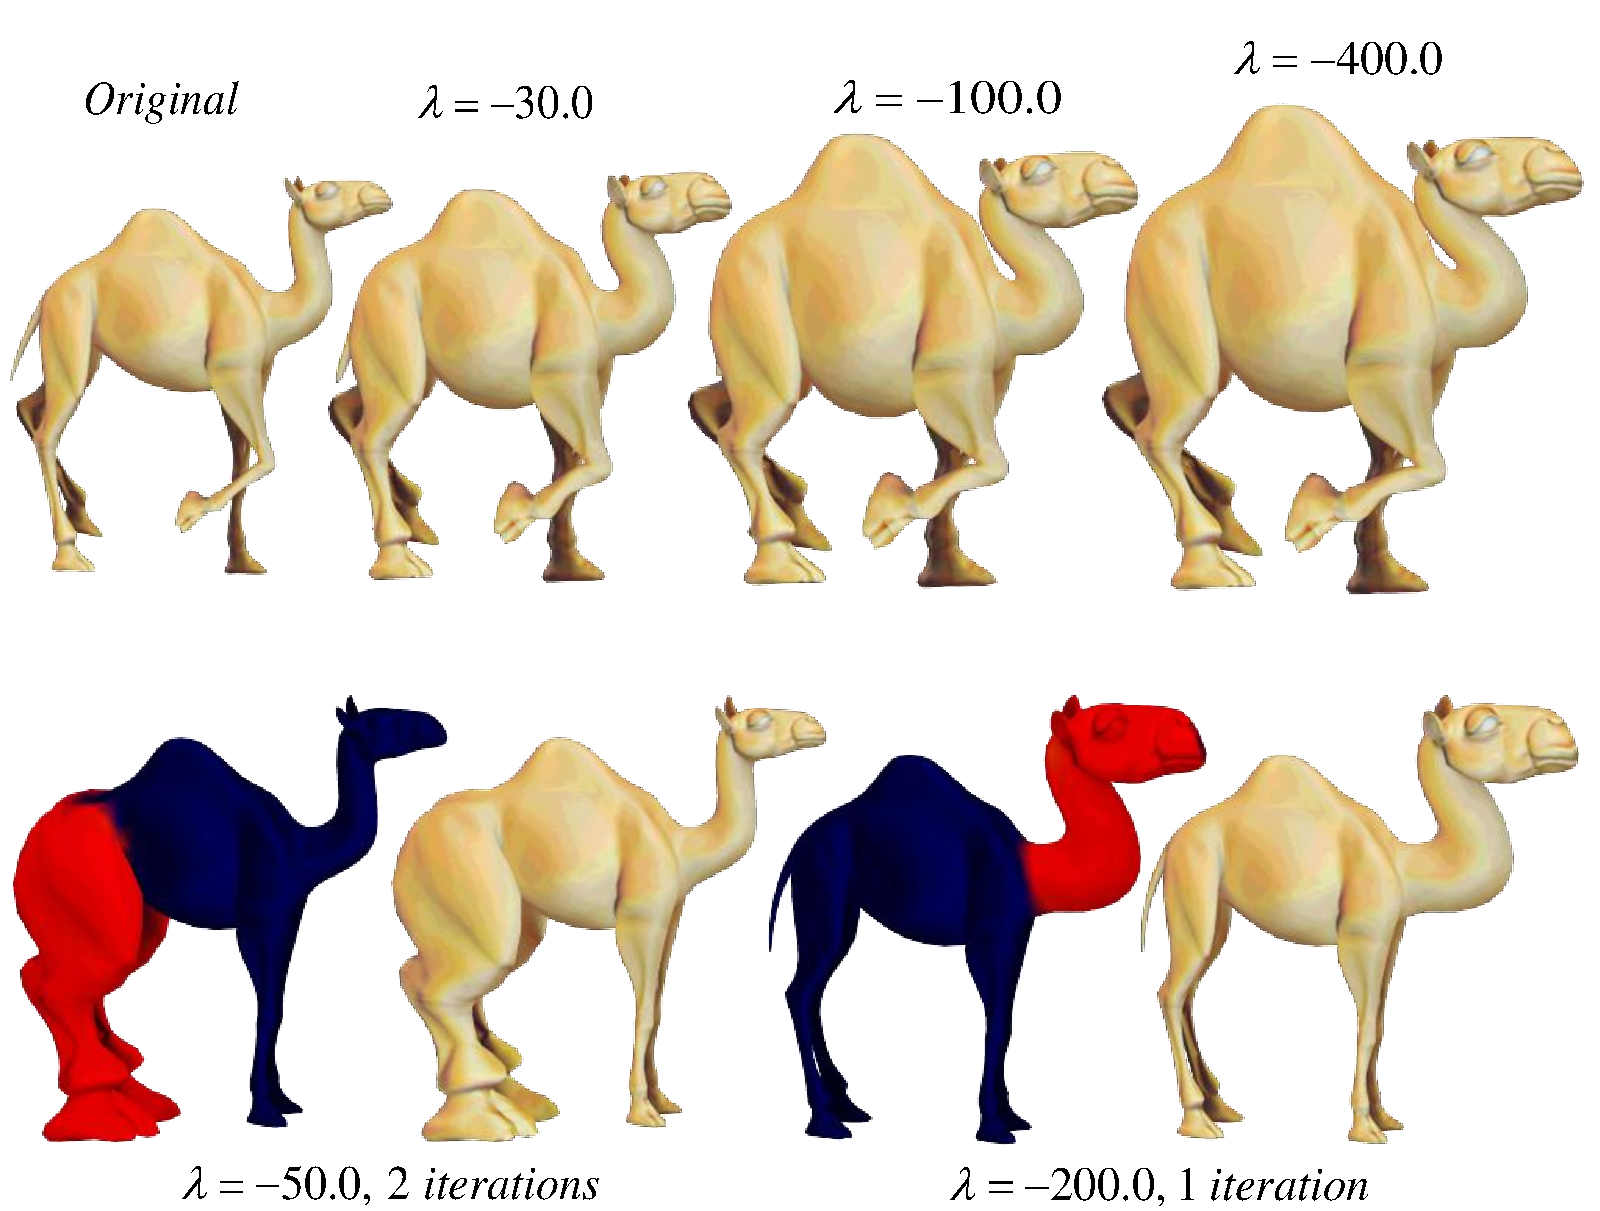
\includegraphics[width=1\columnwidth]{images/camello_enhanced2}

\caption{\label{fig:camello_enhanced}Top row: Original camel model in left.
Shape enhancement with $\lambda=-30.0$, $\lambda=-100.0$, $\lambda=-400.0$.
Bottom row: Shape enhancement with weight vertex group, $\lambda=-50.0$
and 2 iterations for the legs, $\lambda=-200.0$ and 1 iteration for
the head and neck.}
\end{figure}


The enhancement of the silhouette features is predictable and invariant
under isometric transformations, as those classically used in some
animations (see Figure \ref{fig:Animated_Camell}). In this figure,
the animation shows some camel poses during a walk, the enhancement
is performed at the neck and legs, as shown in the bottom left camel
in figure \ref{fig:Animated_Camell}. Local modifications produced
by the pose interpolation or animation rigging practically do not
affect the result. In spite of at any pose of the camel legs there
is a clear difference, the enhancement method allows a flesh-like
shape in the original pattern produced by the artist. This is due
to the mesh restricted diffusion process so that small local changes
are treated without affecting the global solution. The method therefore
is rotation invariant since it depends exclusively on the normal mesh
field, which is rotation invariant. 

Figure \ref{fig:Sculpt_Brush} shows the use of a shape enhancement
brush for sculpting in real time. One pass was used with the brush,
as shown in the figure, with the blue and red radius. In figure \ref{fig:Sculpt_Brush}.b
the camel foot shows the inflation intersection that looks like two
bubbles, a similar pattern to what is observed to the fingers on the
bottom of the same figure. The silhouette enhancement is observed
in figure \ref{fig:Sculpt_Brush}.c since the main shape is retained
together with its finger and foot details. Similar results can be
obtained by a user, however it would take several steps and require
the use of several brushes, while the shape enhancement took a single
step. Likewise, this new method can easily enhance organic features
like muscles during the sculpting process. In figure \ref{fig:Performance-sculpt}
the shape enhancement brush performance is illustrated, in this experiment
three models with 12K, 40K and 164K vertices, were used. These models
were sculpted with the shape enhance brush, at each step the brush
sphere containing a variable number of vertices for processing. The
processing time for 800 vertices in the camel paw (40k model) only
took 0.1 seconds, for 2600 vertices in the leg and neck (model 40k)
took 0.5 seconds, these times are suitable in real applications since
an artist sculpts a model for parts, and each part is represented
by an average of about 1800 vertices.

Tests with the Laplacian operator (equation \ref{eq:TQLBO_Simple_Matrix})
and its normalized version (equation \ref{eq:TQLBO-Normalized_Matrix}),
produce similar results if the triangles or quads that compose the
mesh are about the same size. The normalized version is more stable
and predictable because it is not divided by the area of the ring
which may be very small and causes numeric problems, as shown in figure
\ref{fig:(a)Monkey}.c bottom row. The shape enhancement of the model
with the normalized Laplacian operator results in a more regular pattern.
The model can be deformed with a TQLBO normalized version with large
$\lambda$ ($\lambda>400$) while intersecting itself with no peaks.
Figure \ref{fig:(a)Monkey}.c shows different results due to the quads
areas in the model. Quadss with larger area have smaller enhancement
(figure \ref{fig:(a)Monkey}.c skull), and smaller quads have larger
enhancements (figure \ref{fig:(a)Monkey}.c chin).

\begin{figure}
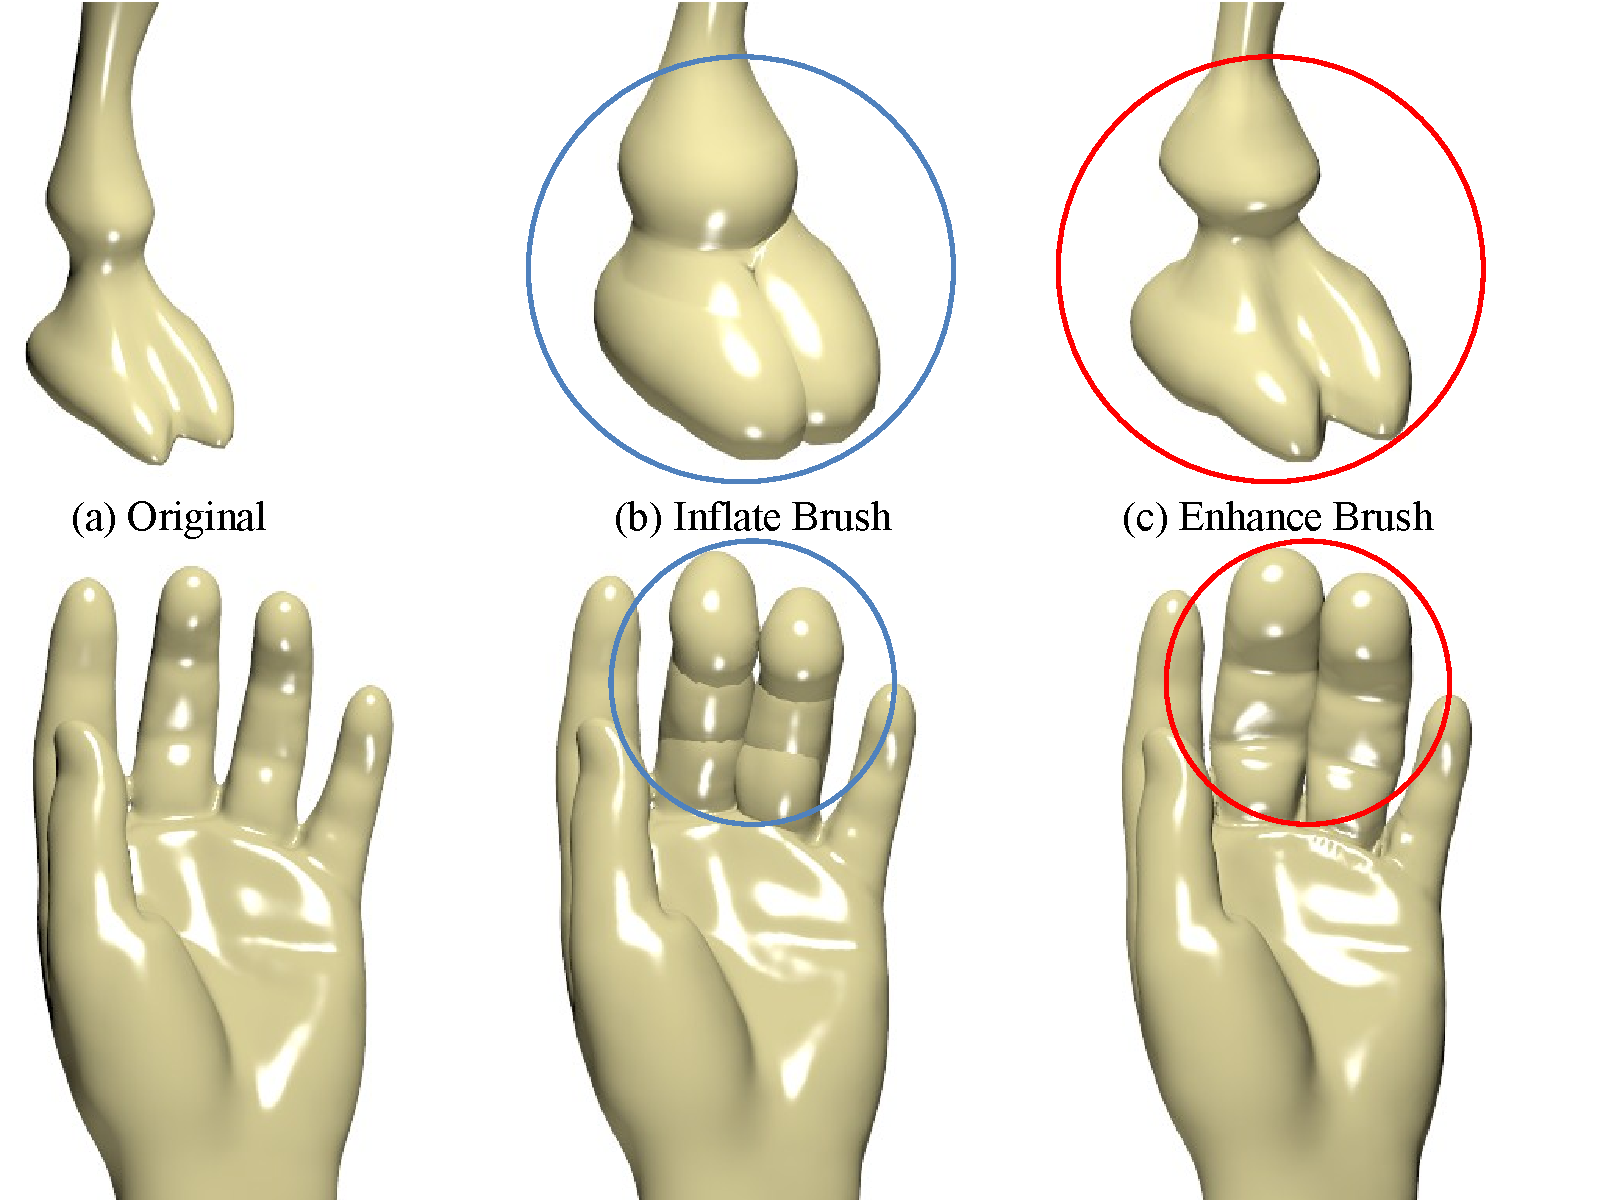
\includegraphics[width=1\columnwidth]{images/sculpt_brush}

\caption{\label{fig:Sculpt_Brush}Top row: (a) Leg Camel, (b) Inflate brush
for leg into blue circle, (c) Enhance shape brush for leg into red
circle. Bottom row: (a) Hand, (b) Inflate brush for fingers into blue
circle, (c) Shape enhancement brush for fingers in red circle.}
\end{figure}


\begin{figure}
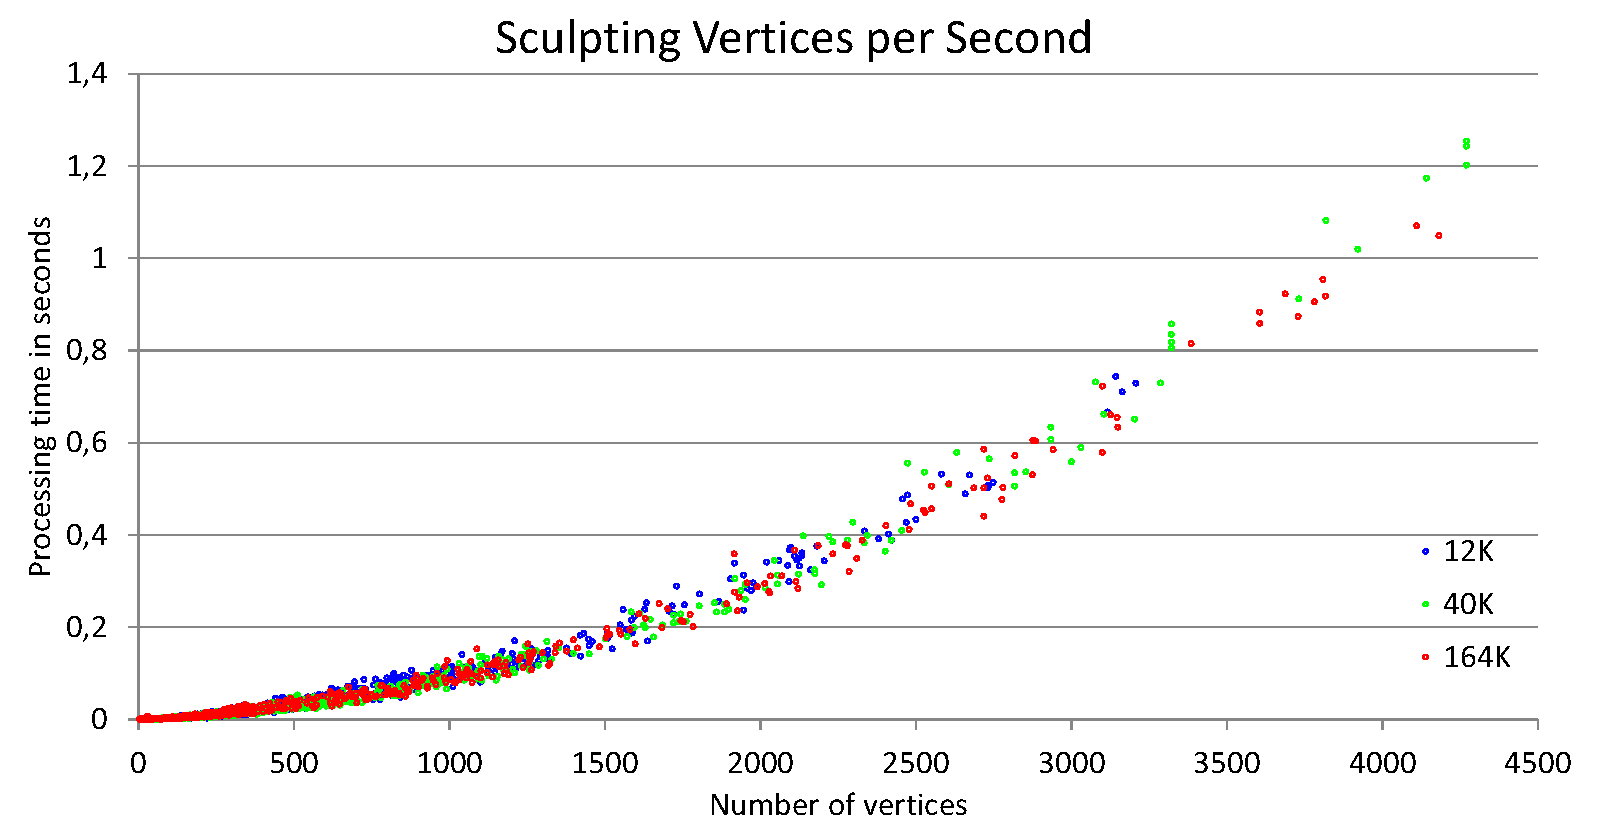
\includegraphics[width=1\columnwidth]{images/verts_per_second_sculpt}

\caption{\label{fig:Performance-sculpt}Performance of our dynamic shape enhancement
brush in terms of the sculpted vertices per second. Three models with
12K, 40K, 164K vertices used for sculpting in real time.}
\end{figure}


\begin{figure}
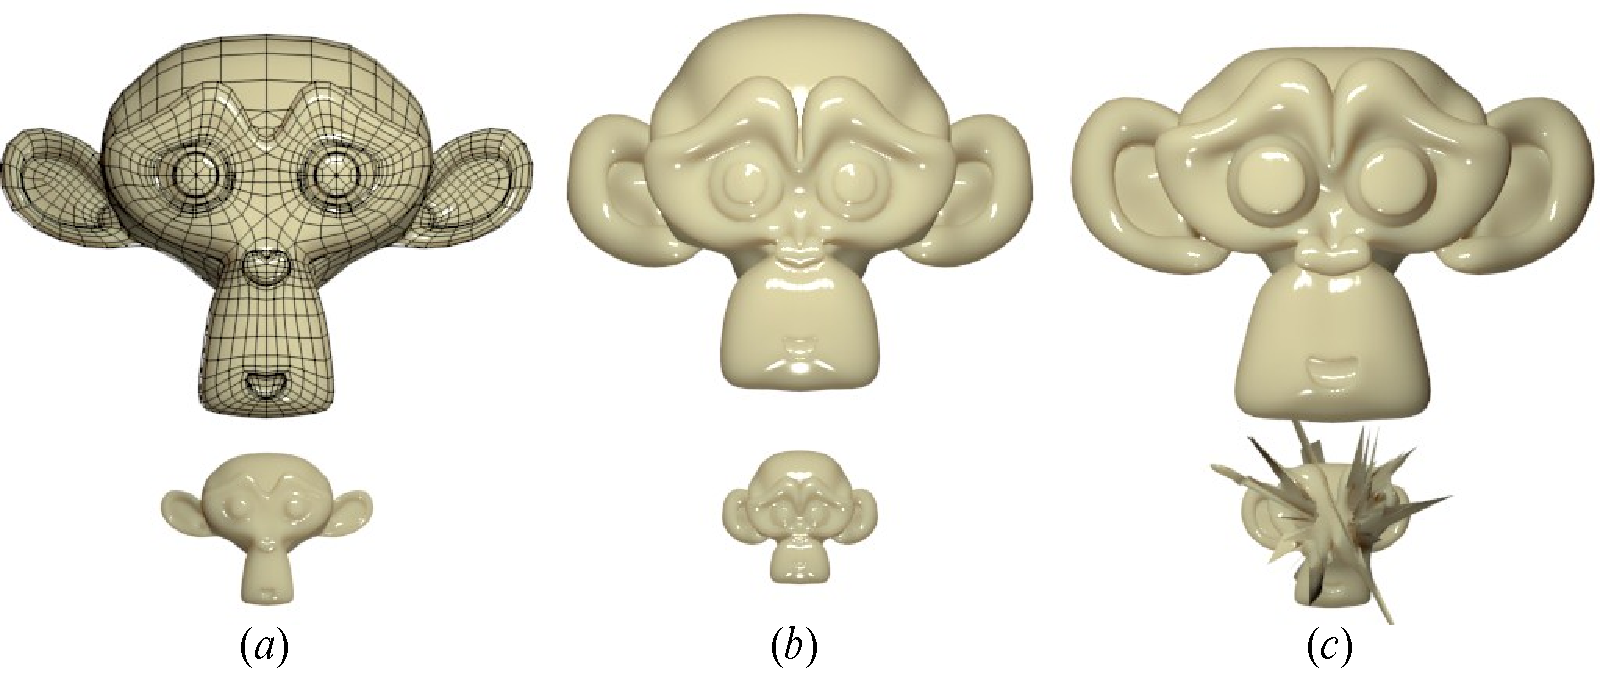
\includegraphics[width=1\columnwidth]{images/monkey}

\caption{\label{fig:(a)Monkey}(a) Bottom row: Original Model. Top row: Original
model scaled by 4. (b) Top and bottom row: enhancing with Normalized-TQLBO
$\lambda=-50$ (c) Top and bottom row: enhancing with TQLBO $\lambda=-50$.}
\end{figure}


\begin{figure*}[t]
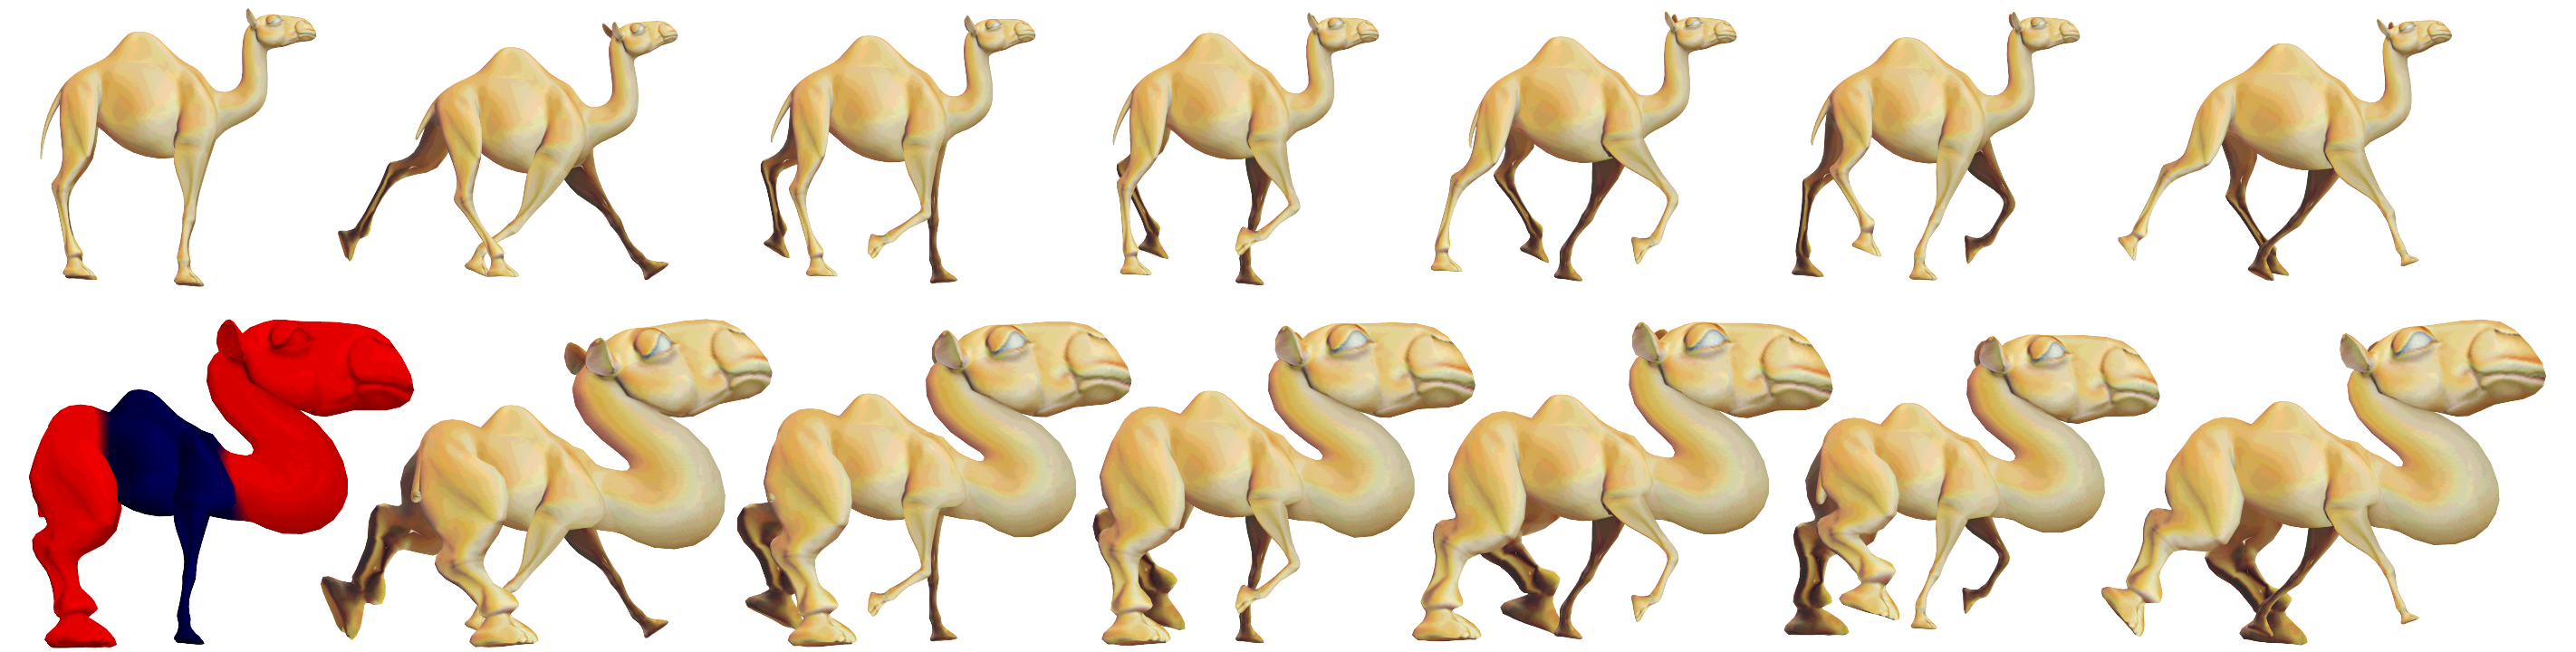
\includegraphics[width=1\textwidth]{images/camello_walk2}

\caption{\label{fig:Animated_Camell}The method is pose insensitive. The enhancement
for the different poses are similar in terms of shape. Top row: Original
walk cycle camel model. Bottom row: Shape enhancement with weight
vertex group, $\lambda=-400$ and $2$ iterations. }
\end{figure*}



\subsection{Implementation\label{sub:Implementation}}

The method was implemented as a modifier for modeling and brush for
sculpting, on the Blender software \cite{blender} in C and C++. Working
with the Blender allowed to test the method interactively against
others, as Catmull-Clark, weight vertex groups and sculpting system
in Blender.

To improve the performance, it was worked with the Blender mesh struct,
visiting each triangle or quad and storing its corresponding index
and the sum of the Laplacian weights of the ring in a list so that
only two visits were required for the list of mesh faces and two times
the edge list, if the mesh was not closed. This drastically reduced
calculations, enabling real-time processing. In the construction of
the Laplacian matrix, several index were locked at vertices having
face areas or edge lengths with zero value that could cause spikes
and bad results.

Under these conditions, the matrix at equation \ref{eq:TQLBO_Simple_Matrix}
is sparse since the number of neighbors per vertex, corresponding
to the number of data per row, is smaller compared to the total number
of vertices in the mesh. To solve the linear system equation \ref{eq:Lineal_System_with_wp}
was used OpenNL which is a a library for solving sparse linear system.


\section{Conclusion and future work\label{sec:Conclusion-and-future}}

This work presented an extension of the Laplace Beltrami operator
for hybrid quad/triangle meshes that can be used in production environments
and provides results similar to those obtained by working only with
triangles or quads. This paper has introduced a new way to change
silhouettes in a mesh for modeling or sculpting in a few steps by
means of the curvature model modification while preserving its overall
shape. In addition, a new modeling method has also been presented
some possible applications have been illustrated. The method works
properly with isometric transformations, opening the possibility of
introducing it on the process of animation.

We show that this tool may work in early modeling stages, case in
which coarse models are used, allowing to modify the shape generated
by the Catmull-Clark subdivision surfaces, and thereby avoiding edition
of the vertices with change of a single parameters.

Future work includes the analysis of theoretical relationships between
the Catmull-Clark subdivision surfaces and the Laplacian smoothing
since they can produce very similar results. 


\section*{Acknowledgments}

We wold like to thank  anonymous friends for their support of our
research. 

This work was supported in part by the Blender Foundation, Google
Summer of code program at 2012. 

Livingstone elephant model is provided courtesy of INRIA and ISTI
by the AIM@SHAPE Shape Repository. Hand model is courtesy of the FarField
Technology Ltd. Camel model by Valera Ivanov is licensed under a Creative
Commons Attribution 3.0 Unported License. Dinosaur and Monkey models
are under public domain, courtesy of Blender Foundation.

\bibliographystyle{acmsiggraph/acmsiggraph}
\bibliography{template}
 
\end{document}
